\documentclass{article}

%% Page Margins %%
\usepackage{geometry}
\geometry{
    top = 0.75in,
    bottom = 0.75in,
    right = 0.75in,
    left = 0.75in,
}

\usepackage{amsmath}
\usepackage{graphicx}
\usepackage{parskip}

\title{Lab 6: Finite State Machines}

% TODO: Enter your name
\author{Qianjun Huang}

\begin{document}
\maketitle

\section{Part I}

\begin{enumerate}

\item Complete Table~\ref{t:part1_state_encodings} below.

\begin{table}[ht!]
\caption{State Encodings}
\label{t:part1_state_encodings}
\centering
\begin{tabular}{|l|l|}
\hline
State & Encoding \\ \hline
A & 0000001\\ \hline
B & 0000010\\ \hline
C & 0000100\\ \hline
D & 0001000\\ \hline
E & 0010000\\ \hline
F & 0100000\\ \hline
G & 1000000\\ \hline
\end{tabular}
\end{table}

\item Complete Table~\ref{t:part1_encoded_transition_table} below.

\begin{table}[ht!]
\caption{Encoded State Transition Table for Robo-Snail II}
\label{t:part1_encoded_transition_table}
\centering
\begin{tabular}{|l|l|l|}
\hline
Current State & W & Next State \\ \hline
0000001 & 0 & 0000001\\
0000001 & 1 & 0000010\\
0000010 & 0 & 0000001\\
0000010 & 1 & 0000100\\
0000100 & 0 & 0010000\\
0000100 & 1 & 0001000\\
0001000 & 0 & 0010000\\
0001000 & 1 & 0100000\\
0010000 & 0 & 0000001\\
0010000 & 1 & 1000000\\ 
0100000 & 0 & 0010000\\
0100000 & 1 & 0100000\\
1000000 & 0 & 0000001\\
1000000 & 1 & 0000100\\
\hline
\end{tabular}
\end{table}

\item Derive equations for each of your next state outputs below.

\begin{align*}
    S'_0 &= S_0\Bar{W} + S_1\Bar{W} + S_4\Bar{W} + S_6\Bar{W}\\
    S'_1 &= S_0W\\
    S'_2 &= S_1W + S_6W\\
    S'_3 &= S_2W\\
    S'_4 &= S_2\Bar{W} + S_3\Bar{W} + S_5\Bar{W}\\
    S'_5 &= S_3W + S_5W\\
    S'_6 &= S_4W\\
\end{align*}

\item Export the subcircuit schematic as an image and include it in your report.

\begin{figure}[ht!]
    \centering
    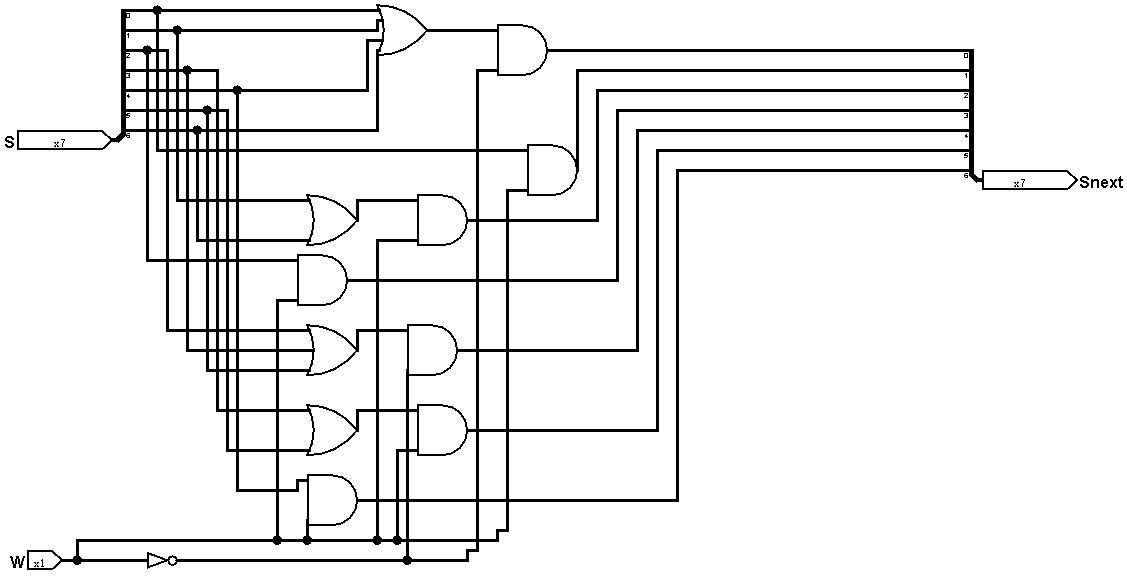
\includegraphics[width=0.3\textwidth]{lab6_part1_next_state.png}
    \caption{A schematic of Part I's next\_state.}
    \label{f:part1_next_state}
\end{figure}

\item Complete Table~\ref{t:part1_output_table} below.

\begin{table}[ht!]
\caption{Encoded Output Table for Robo-Snail II}
\label{t:part1_output_table}
\centering
\begin{tabular}{|l|l|}
\hline
State   & Output \\ \hline
0000001 & 0\\ \hline
0000010 & 0\\ \hline
0000100 & 0\\ \hline
0001000 & 0\\ \hline
0010000 & 0\\ \hline
0100000 & 1\\ \hline
1000000 & 1\\ \hline
\end{tabular}
\end{table}

\item Derive the equation for your output logic below.

$$Z = S_5 + S_6$$

\item Export the subcircuit schematic as an image and include it in your report.

\begin{figure}[ht!]
    \centering
    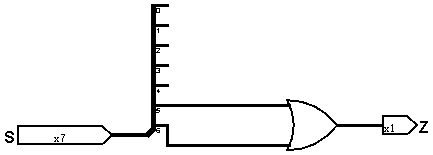
\includegraphics[width=0.5\textwidth]{lab6_part1_output.png}
    \caption{A schematic of Part I's output\_logic.}
    \label{f:part1_output_logic}
\end{figure}
\end{enumerate}

\clearpage
\section{Part II}

\begin{enumerate}
\item Complete Table~\ref{t:part2_encoded_transition_table} below.

\begin{table}[ht!]
\caption{Encoded State Transition Table for Part II}
\label{t:part2_encoded_transition_table}
\centering
\begin{tabular}{|l|l|}
\hline
Current State & Next State \\ \hline
0000 & 0001\\
0001 & 0010\\
0010 & 0011\\
0011 & 0100\\
0100 & 0000\\
\hline
\end{tabular}
\end{table}
\item Complete Table~\ref{t:part2_output_table} below.

\begin{table}[ht!]
\caption{Output Table for Part II}
\label{t:part2_output_table}
\centering
\begin{tabular}{|l|l|l|l|l|l|l|l|}
\hline
S & ALUSelB & ALUop & LoadC & LoadALUout & LoadA & LoadB & LoadR\\ \hline
0000 & 00 & 0 & 1 & 0 & 0 & 0 & 0\\
0001 & 00 & 0 & 0 & 0 & 1 & 0 & 0\\
0010 & 00 & 1 & 0 & 1 & 1 & 0 & 0\\
0011 & 10 & 0 & 0 & 1 & 0 & 1 & 0\\
0100 & 01 & 0 & 0 & 0 & 0 & 0 & 1\\

\hline
\end{tabular}
\end{table}

\item Draw the state transition diagram and include it in Figure~\ref{f:part2_state_diagram}.

\begin{figure}[ht!]
    \centering
    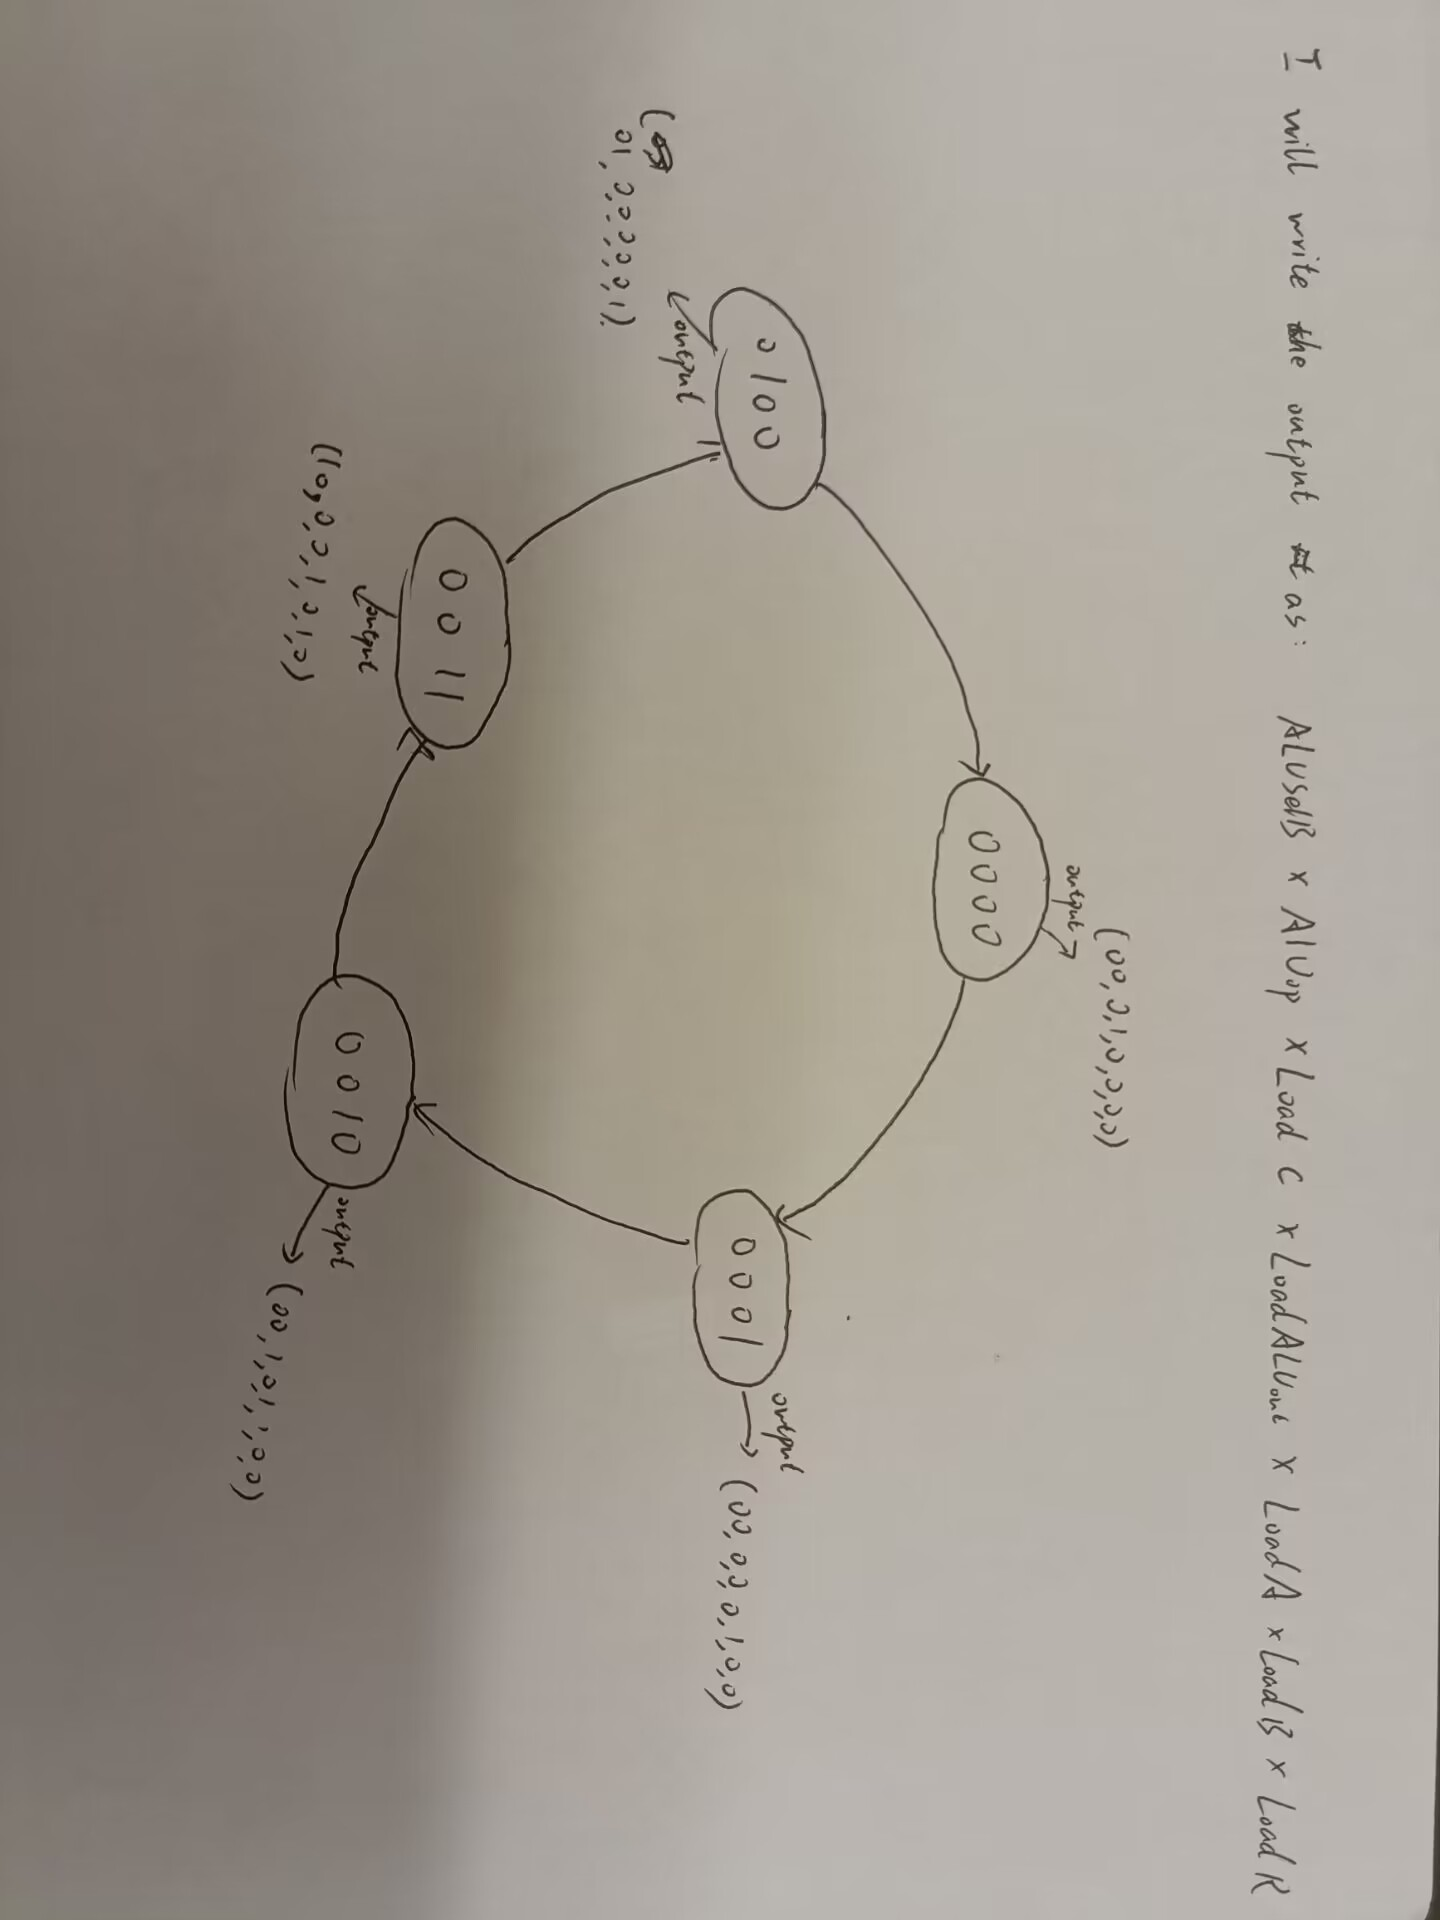
\includegraphics[width=0.3\textwidth]{lab6_part2_state_diagram.png}
    \caption{The state transition diagram for Part II}
    \label{f:part2_state_diagram}
\end{figure}

\item Describe how each state controls the datapath from Part II in Table~\ref{t:part2_state_descriptions}.

\begin{table}[ht!]
\caption{A description of how a state controls the datapath}
\label{t:part2_state_descriptions}
\centering
\begin{tabular}{|l|l|}
\hline
State & Description\\ \hline
0000 & Load the value of Input(C) to RegC\\ \hline
0001 & Load the value of Input(A) to RegA\\ \hline
0010 & RegA and RegA are two operands and the operation of ALU is *, and then the output ($A^2$) is loaded in RegA\\ \hline
0011 & RegA and RegC are two operands and the operation of ALU is +, and then the output ($A^2 + C$) is loaded in RegB\\ \hline
0100 & RegA and RegB are two operands and the operation of ALU is +, and then the output ($2A^2 + C$) is loaded in RegR\\
\hline
\end{tabular}
\end{table}

\item Export the timing diagram as an image and include it in your report.

\begin{figure}[ht!]
    \centering
    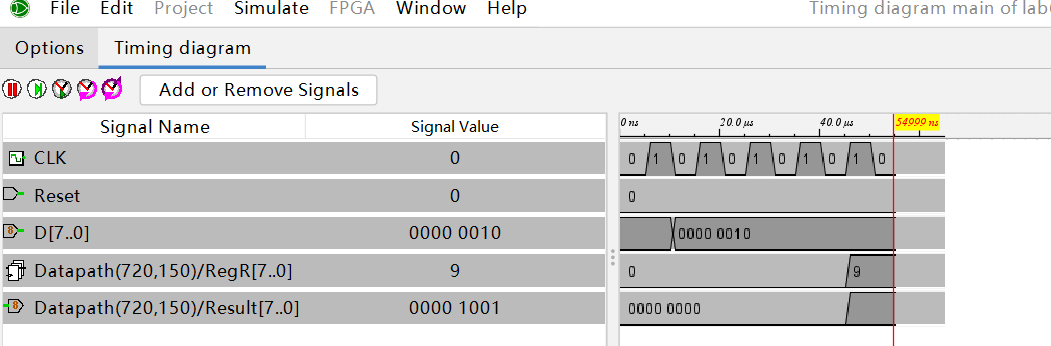
\includegraphics[width=0.65\textwidth]{lab6_part2_timing.png}
    \caption{A timing simulation of the main schematic in Part II.}
    \label{f:part2_timing}
\end{figure}

\end{enumerate}

\end{document}